%%%%%%%%%%%%%%%%%%%%%%%%%%%%%%%%%%%%%%%%%%%%%%%%%%%%%%%%%%%%%%%%%%%%%%%%%%%%%%%%%%%%%%%
%%%%%%%%%%%%%%%%%%%%%%%%%%%%%%%%%%%%%%%%%%%%%%%%%%%%%%%%%%%%%%%%%%%%%%%%%%%%%%%%%%%%%%%
% 
% This top part of the document is called the 'preamble'.  Modify it with caution!
%
% The real document starts below where it says 'The main document starts here'.

\documentclass[12pt]{article}
\usepackage{graphicx}
\usepackage{float}
\usepackage{amssymb,amsmath,amsthm}
\usepackage[top=1in, bottom=1in, left=1.25in, right=1.25in]{geometry}
\usepackage{fancyhdr}
\usepackage{enumerate}

% Comment the following line to use TeX's default font of Computer Modern.
\usepackage{times,txfonts}

\newtheoremstyle{homework}% name of the style to be used
  {18pt}% measure of space to leave above the theorem. E.g.: 3pt
  {12pt}% measure of space to leave below the theorem. E.g.: 3pt
  {}% name of font to use in the body of the theorem
  {}% measure of space to indent
  {\bfseries}% name of head font
  {:}% punctuation between head and body
  {2ex}% space after theorem head; " " = normal interword space
  {}% Manually specify head
\theoremstyle{homework} 

% Set up an Exercise environment and a Solution label.
\newtheorem*{exercisecore}{Exercise \@currentlabel}
\newenvironment{exercise}[1]
{\def\@currentlabel{#1}\exercisecore}
{\endexercisecore}

\newcommand{\localhead}[1]{\par\smallskip\noindent\textbf{#1}\nobreak\\}%
\newcommand\solution{\localhead{Solution:}}

%%%%%%%%%%%%%%%%%%%%%%%%%%%%%%%%%%%%%%%%%%%%%%%%%%%%%%%%%%%%%%%%%%%%%%%%
%
% Stuff for getting the name/document date/title across the header
\makeatletter
\RequirePackage{fancyhdr}
\pagestyle{fancy}
\fancyfoot[C]{\ifnum \value{page} > 1\relax\thepage\fi}
\fancyhead[L]{\ifx\@doclabel\@empty\else\@doclabel\fi}
\fancyhead[C]{\ifx\@docdate\@empty\else\@docdate\fi}
\fancyhead[R]{\ifx\@docauthor\@empty\else\@docauthor\fi}
\headheight 15pt

\def\doclabel#1{\gdef\@doclabel{#1}}
\doclabel{Use {\tt\textbackslash doclabel\{MY LABEL\}}.}
\def\docdate#1{\gdef\@docdate{#1}}
\docdate{Use {\tt\textbackslash docdate\{MY DATE\}}.}
\def\docauthor#1{\gdef\@docauthor{#1}}
\docauthor{Use {\tt\textbackslash docauthor\{MY NAME\}}.}
\makeatother

% Shortcuts for blackboard bold number sets (reals, integers, etc.)
\newcommand{\Reals}{\ensuremath{\mathbb R}}
\newcommand{\Nats}{\ensuremath{\mathbb N}}
\newcommand{\Ints}{\ensuremath{\mathbb Z}}
\newcommand{\Rats}{\ensuremath{\mathbb Q}}
\newcommand{\Cplx}{\ensuremath{\mathbb C}}
%% Some equivalents that some people may prefer.
\let\RR\Reals
\let\NN\Nats
\let\II\Ints
\let\CC\Cplx

%%%%%%%%%%%%%%%%%%%%%%%%%%%%%%%%%%%%%%%%%%%%%%%%%%%%%%%%%%%%%%%%%%%%%%%%%%%%%%%%%%%%%%%
%%%%%%%%%%%%%%%%%%%%%%%%%%%%%%%%%%%%%%%%%%%%%%%%%%%%%%%%%%%%%%%%%%%%%%%%%%%%%%%%%%%%%%%
% 
% The main document start here.

% The following commands set up the material that appears in the header.
\doclabel{Stat 300: Homework 2}
\docauthor{Stefano Fochesatto}
\docdate{\today}

\begin{document}
\begin{enumerate}
\item\hspace{.5in}\textbf{Exercise 1.58:}\\
\\
 A company utilizes two different machines to manufacture parts of a certain type. During a single shift, a sample of $n=20$ parts produced by each machine is obtained, and the value of a particular critical dimension for each part is determined. The comparative boxplot at the bottom of this page is constructed from the resulting data. Compare and contrast the two samples.\\
 \\
 \begin{center}
  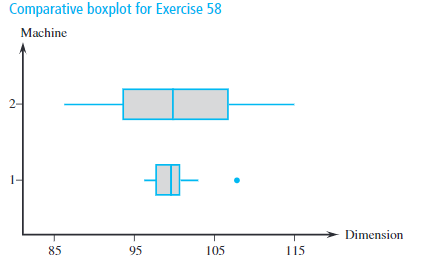
\includegraphics[width = .66\textwidth]{boxplot.png}  
 \end{center}
 

 \textbf{Answer:} Looking at the spread of the 2 boxplots we can make some assertions about the manufacturing quality of each machine.
 Firstly the machine 2 has a larger inter quartile range which means it will produce a less consistent product. 
\vspace{1in}





\item\hspace{.5in}\textbf{Exercise 1.68:}\\
\begin{enumerate}
\item For what value of $c$ is the quantity $\sum (x_i - c)^2$ minimized? [Hint: Take the derivative with respect to $c$, set equal to $0$, and solve.]\\
\\
 \textbf{Answer:}
 Taking the derivative of $f(x) = \sum (x_i - c)^2$, using chain-rule we get that $f'(x) = \sum -2(x_i - c)$. Solving at $f'(x) = 0$,
 \begin{align*}
  0 &=\sum -2(x_i - c)\\
  0 &=-2\sum (x_i - c)\\
  0 &=-nc + \sum (x_i)\\
  nc &= \sum (x_i)\\
  c &=\frac{\sum (x_i)}{n} = \overline{x}
 \end{align*}
 Thus when $c = \overline{x}$, $f(x)$ is minimized.
\vspace{.5in}
\item Using the result of part $(a)$, which of the two quantities $\sum (x_i -\overline{x})^2$ and $\sum(x_i -\mu)^2$ will be smaller than the other (assuming that $\overline{x} \neq \mu$)?\\

 \textbf{Answer:} Recall that $f(x) = \sum (x_i - c)^2$ is minimized when $c = \overline(x)$ thus $\sum (x_i -\overline{x})^2$ must be smaller. Furthermore
 we know that $x_i$ represent our sample, had they represented our population we would say that $\sum(x_i -\mu)^2$ is larger.    
\end{enumerate}
\vspace{1in}










\item\hspace{.5in}\textbf{Exercise 2.6:} \\
\\
A college library has five copies of a certain text on reserve. Two copies ($1$ and $2$) are first printings, and the other three ($3$, $4$, and $5$) are second printings. A student examines these books in random order, stopping only when a second printing has been selected. One possible outcome is $5$, and another is $213$.
\begin{enumerate}
\item List the outcomes in $\mathcal{S}$\\

 \textbf{Answer:}
 \begin{center}
  \begin{tabular}{c c c c c c c}
  3 & 4 & 5 &  &  &  \\
  13 & 23 & 14 & 24 & 15 & 25\\
  123 & 213 & 124 & 214 & 125 & 215 
  \end{tabular}
\end{center}
\vspace{.5in}
 
\item Let $A$ denote the event that exactly one book must be examined. What outcomes are in $A$?\\

\textbf{Answer:}
\begin{center}
 \begin{tabular}{c c c c c c c}
 3 & 4 & 5 &  &  &  
 \end{tabular}
\end{center}
\vspace{.5in}

\item Let $B$ be the event that book $5$ is the one selected. What outcomes are in $B$?\\
\textbf{Answer:}
\begin{center}
 \begin{tabular}{c c c }
  5 &  \\
  15 & 25\\
  125 & 215 
 \end{tabular}
\end{center}
\vspace{.5in}


\item Let $C$ be the event that book $1$ is not examined. What outcomes are in $C$?\\
\textbf{Answer:}
\begin{center}
 \begin{tabular}{c c c c}
 3 & 4 & 5 \\
 23 & 24 & 25
 \end{tabular}
\end{center}


\end{enumerate}
\vspace{1in}

\item\hspace{.5in}\textbf{Exercise 2.12:}\\
\\
Consider randomly selecting a student at a large university, and let $A$ be the event that the selected student has a Visa card and $B$ be the analogous event for MasterCard. Suppose that $P(A)= .6$ and $P(B) = .4$.
\begin{enumerate}
\item Could it be the case that $P(A \cap B) = .5$? Why or why not? [Hint: See Exercise $24$.]\\
\\
 \textbf{Answer:} It is not the case that that $P(A \cap B) = .5$, since by set theory we know that $P(A \cap B) \leq min(P(A), P(B))$.
 \\
\item From now on, suppose that $P(A \cap B) = .3$. What is the probability that the selected student has at least one of these two types of cards?\\
\\
 \textbf{Answer:} Through inclusion exclusion we know that $P(A \cup B) = P(A) + P(B) - P(A \cap B) = .6 + .4 - .3 = .7$. 
 \\
\item What is the probability that the selected student has neither type of card?\\
\\
 \textbf{Answer:} Note that $P(\overline{A \cap B}) = 1 - P(A \cup B) = 1 - .7 = .3$.
 \\
\item Describe, in terms of $A$ and $B$, the event that the selected student has a Visa card but not a MasterCard, and then calculate the probability of this event.\\
\\
 \textbf{Answer:} The event $P(A\setminus B) = P(A) - P(A \cap B) = .6 - .3 = .3$.
 \\
\item Calculate the probability that the selected student has exactly one of the two types of cards.\\
\\
 \textbf{Answer:} The event $P((A \cup B) - (A \cap B)) = P(A \cup B) - P(A \cap B) = .7  - .3 = .4$.
 \\
\end{enumerate}
\vspace{1in}


\item\hspace{.5in}\textbf{Exercise 2.16:}\\
\\
An individual is presented with three different glasses of cola, labeled $C$, $D$, and $P$. He is asked to taste all three and then list them in order of preference. Suppose the same cola has actually been put into all three glasses.
\begin{enumerate}
\item What are the simple events in this ranking experiment, and what probability would you assign to each one?\\

\textbf{Answer:}
\begin{center}
 \begin{tabular}{c c c c}
 CDP & PCD & DCP \\
 CPD & PDC & DPC
 \end{tabular}
\end{center}
Since it's equally likely that the individual produces any of these rankings each event would have a probability of $\frac{1}{6}$.

\item What is the probability that $C$ is ranked first?\\
\\
 \textbf{Answer:} The probability that $C$ is ranked first is $\frac{1}{3}$.
 \\
\item What is the probability that $C$ is ranked first and $D$ is ranked last?\\
\\
 \textbf{Answer:} The probability that $C$ is ranked first and $D$ is ranked last is $\frac{1}{6}$.
 \\
\end{enumerate}
\vspace{1in}


\item\hspace{.5in}\textbf{Exercise 2.24:}\\
\\
Show that if one event $A$ is contained in another event $B$ (i.e., $A$ is a subset of $B$), then $P(A) \leq P(B).$ [Hint: For such $A$ and $B$, $A$ and $B\cap A'$ are disjoint and $B= A \cup (B \cap A')$, as can be seen from a Venn diagram.] For general $A$ and $B$, what does this imply about the relationship among $P(A\cap B)$, $P(A)$ and $P(A \cup B)$?\\
\\
 \textbf{Answer:} Recall that if two sets $A$ and $B$ are disjoint then $P(A\cup B) = P(A) +P(B)$. by set theory we know that,
 \begin{align*}
   P(B) &= P(A \cup (B\cap\overline{A}))\\
   &= P(A) + P(B\cap\overline{A})\\
   &\geq P(A)
 \end{align*}
Thus we have shown that if $A \subseteq B$ then $P(B) \geq P(A)$. Furthermore since $A$ is contained in $B$ we know the following, $P(A \cap B) = P(A)$, $P(A \cup B) = P(B)$




\vspace{1in}


\item\hspace{.5in}\textbf{Exercise 2.32:}\\
\\
An electronics store is offering a special price on a complete set of components (receiver, compact disc player, speakers, turntable). A purchaser is offered a choice of manufacturer for each component:\\
\\
\textbf{Receiver:} Kenwood, Onkyo, Pioneer, Sony, Sherwood \\
\textbf{Compact disc player:} Onkyo, Pioneer, Sony, Technics\\
\textbf{Speakers:} Boston, Infinity, Polk\\
\textbf{Turntable:} Onkyo, Sony, Teac, Technics\\
\\
A switchboard display in the store allows a customer to hook together any selection of components (consisting of one of each type). Use the product rules to answer the following questions:
\begin{enumerate}
\item In how many ways can one component of each type be selected?\\
\\
 \textbf{Answer:} Using the multiplication rule we know that there are, 
 \begin{equation*}
   5*4*3*4 = 240.
 \end{equation*}
 So there are 240 different ways to select one component of each type.
 \\
\item In how many ways can components be selected if both the receiver and the compact disc player are to be Sony?\\
\\
 \textbf{Answer:} Using the multiplication rule again we can see that there are $3*4 = 12$ ways to select the rest of the components.
 \\
\item In how many ways can components be selected if none is to be Sony?\\
\\
 \textbf{Answer:} Using the multiplication rule we see that there are $3*3*3*4 = 144$ ways to select the 4 audio components when none of them are Sony.
 \\
\item In how many ways can a selection be made if at least one Sony component is to be included?\\
\\
 \textbf{Answer:} Using Inclusion-exclusion we know that we can subtract the number of selections with no Sony components from the total number of selections to get the number of selections with atleast one Sony component.
 \begin{equation*}
  240 - 144 = 96.
\end{equation*}
Thus there are $96$ ways to select audio components where atleast one of the 4 is made by Sony.
 \\
\item If someone flips switches on the selection in a completely random fashion, what is the probability that the system selected contains at least one Sony component? Exactly one Sony component?\\
\\
 \textbf{Answer:}The probablilty that the selection contains at least one Sony product is $\frac{96}{240}$. The total number of selections with exactly one sony product is $3*3*4+4*3*4 = 84$ and thus the probability is $\frac{84}{240}$
 \\
\end{enumerate}
\vspace{1in}


\item\hspace{.5in}\textbf{Exercise 2.38:} \\
\\
A sonnet is a $14$-line poem in which certain rhyming patterns are followed. The writer Raymond Queneau published a book containing just $10$ sonnets, each on a different page. However, these were structured such that other sonnets could be created as follows: the first line of a sonnet could come from the first line on any of the $10$ pages, the second line could come from the second line on any of the $10$ pages, and so on (successive lines were perforated for this purpose).
\begin{enumerate}
\item How many sonnets can be created from the $10$ in the book?\\
\\
 \textbf{Answer:} For each of the 14 lines in the sonnet we know that there are 10 lines to choose from. Using the multiplication rule we get that $10^{14}$ sonnets can be created. 
 \\
\item If one of the sonnets counted in part $(a)$ is selected at random, what is the probability that none of its lines came from either the first or the last sonnet in the book?\\
\\
 \textbf{Answer:} The probablity that a selected sonnet has none of it's lines from the first or last sonnet is $\frac{8^{14}}{10^{14}} = .044$.
 \\
\end{enumerate}
\vspace{1in}


\item\hspace{.5in}\textbf{Exercise 2.40:} \\
\\
Three molecules of type $A$, three of type $B$, three of type $C$, and three of type $D$ are to be linked together to form a chain molecule. One such chain molecule is $ABCDABCDABCD$, and another is $BCDDAAABDBCC$.
\begin{enumerate}
\item How many such chain molecules are there? [Hint: If the three $A$’s were distinguishable from one another-- $A_1$, $A_2$, $A_3$ -- and the $B$’s, $C$’s, and $D$’s were also, how many molecules would there be? How is this number reduced when the subscripts are removed from the $A$’s?]\\
\\
 \textbf{Answer:} For the case where each molecule is unique we can simply permute them to find the total number of chain molecules possible, so $12! = 479,001,600$. In the case the subscript is removed we would use a chain combination statement, so $ {12 \choose 3 3 3 3}  = 369,600$
 \\
\item Suppose a chain molecule of the type described is randomly selected. What is the probability that all three molecules of each type end up next to one another (such as in $BBBAAADDDCCC$)?\\
\\
 \textbf{Answer:} We can count the total number of chain molecules where each type is next to each other with $4! = 24$ since all we are really doing is deciding the order of molecule type. Thus the probability that a chain molecule has each type grouped together is $\frac{24}{369,600} = 6.494 *10^{-5}$
 \\
\end{enumerate}
\vspace{1in}


\item\hspace{.5in}\textbf{Exercise 2.52:} \\
\\
A system consists of two identical pumps, $\#1$ and $\#2$. If one pump fails, the system will still operate. However, because of the added strain, the remaining pump is now more likely to fail than was originally the case. That is, $r = P(\#2 \text{ fails} | \#1 \text{ fails})>P(\#2 \text{ fails}) = q$. If at least one pump fails by the end of the pump design life in $7\%$ of all systems and both pumps fail during that period in only $1\%$, what is the probability that pump $\#1$ will fail during the pump design life?\\
\\
 \textbf{Answer:} Suppose that $A$ is the event that pump $\#1$ fails and $B$ is the even that pump $\#2$ fails. We are given that $P(A \cup B) = .07$, $P(A \cap B) = .01$, and $P(B|A) > P(B)$. Since the pumps are identical we know that $P(A) = P(B)$ and since the system will still operate if one pump fails,  $P(B|A) = P(A|B)$ . Let $r = P(B|A) = P(A|B)$ and $q = P(B) = P(A)$. Recall the multiplication rule, 
 \begin{equation*}
   P(A \cap B) = P(A|B)P(B).
 \end{equation*}
By substitution we get that,
\begin{equation*}
  .01 = rq.
\end{equation*}
Through set theory we know that,
\begin{equation*}
  P(A \cup B) = P(A \cap B) + P(B\setminus A) + P(A \setminus B).
\end{equation*}
Recall that,
\begin{equation*}
  P(B\setminus A) = P(B\cap \overline{A}) = P(\overline{A}|B)P(B) = (1-r)q.
\end{equation*}
Through substitution we know that,
\begin{align*}
  .07 &= rq + (1-r)q + (1-r)q, \\
    &= rq + 2(1-r)q.
\end{align*}
Solving this system of equations we get that $r = .25$ and $q = .04$. Thus the probability that pump $\#1$ will fail is $P(A) = .04$.



\vspace{1in}


\item\hspace{.5in}\textbf{Exercise 2.60:} \\
\\
Seventy percent of the light aircraft that disappear while in flight in a certain country are subsequently discovered. Of the aircraft that are discovered, $60\%$ have an emergency locator, whereas $90\%$ of the aircraft not discovered do not have such a locator. Suppose a light aircraft has disappeared.
\begin{enumerate}
\item If it has an emergency locator, what is the probability that it will not be discovered?\\
\\
 \textbf{Answer:} Let $A$ be the event in which an aircraft is discovered. Let $B$ be the event in which an aircraft has an emergency locator. We are 
 given that $P(A) = .70$, $P(B|A) = .60$ and $P(\overline{B}|\overline{A}) = .90$. The probability that an aircraft is not discovered given it has an emergency locator is $P(\overline{A}|B)$. Applying Bayes' Theorem we get,
 \begin{align*}
  P(\overline{A}|B) &= \frac{P(B|\overline{A})P(\overline{A})}{P(B|\overline{A})P(\overline{A})*P(B|A)P(A)},\\
 &= \frac{(1 - .90)(1 - .70)}{(1 - .90)(1 - .70)+(.60)(.70)},\\
 &= \frac{(.10)(.30)}{(.10)(.30)+(.60)(.70)},\\
 &= \frac{.03}{.54},\\
 &= .067.
 \end{align*}
 \\
\item If it does not have an emergency locator, what is the probability that it will be discovered?\\
\\
 \textbf{Answer:} The probability that an aircraft is discovered given that it does not have an emergency locator is $P(A|\overline{B})$. Using Bayes' Theorem again, we know that,
 \begin{align*}
   P(A|\overline{B}) &= \frac{P(\overline{B}|A)P(A)}{P(\overline{B}|A)P(A)+P(\overline{B}|\overline{A})P(\overline{A})},\\
   &= \frac{(1 - .60)(.7)}{(1 - .60)(.7)+(.90)(1-.70)},\\
   &= \frac{(.40)(.7)}{(.40)(.7)+(.90)(.30)},\\
   &= \frac{.28}{.55},\\
   &= .509.\\
 \end{align*}
 \\
\end{enumerate}
\vspace{1in}



\end{enumerate}
\end{document}